\section{Métodologia de Trabalho}
Para o bom desenrolar das atividades de desenvolvimento, é de fundamental importância o estebelecimento de um método de trabalho claro para que todos \textit{stakeholders} consigam constribuir sem \textit{overheads} de compatibilização de trabalhos e/ou conflitos.

Assim, faz-se aqui uma proposta de método de trabalho baseada em princípios das metodologias ágeis.
\subsection{Estratégia de versionamento}
A estratégia de versionamento proposta é uma variação do conhecido \textit{workflow} \textit{gitFlow}%
\footnote{\textit{Git Flow: a successful branching model}, modelo de versionamento proposto por Vincent Driessen, da nvie (\url{http://nvie.com/}), em Janeiro de 2010 e que faz muito sucesso. \url{http://nvie.com/posts/a-successful-git-branching-model/} - Acessado em 01/03/2015}, que pode ser observado na Figura \ref{fig:gitflow}.

    \begin{figure}[htb]%
        \begin{center}
            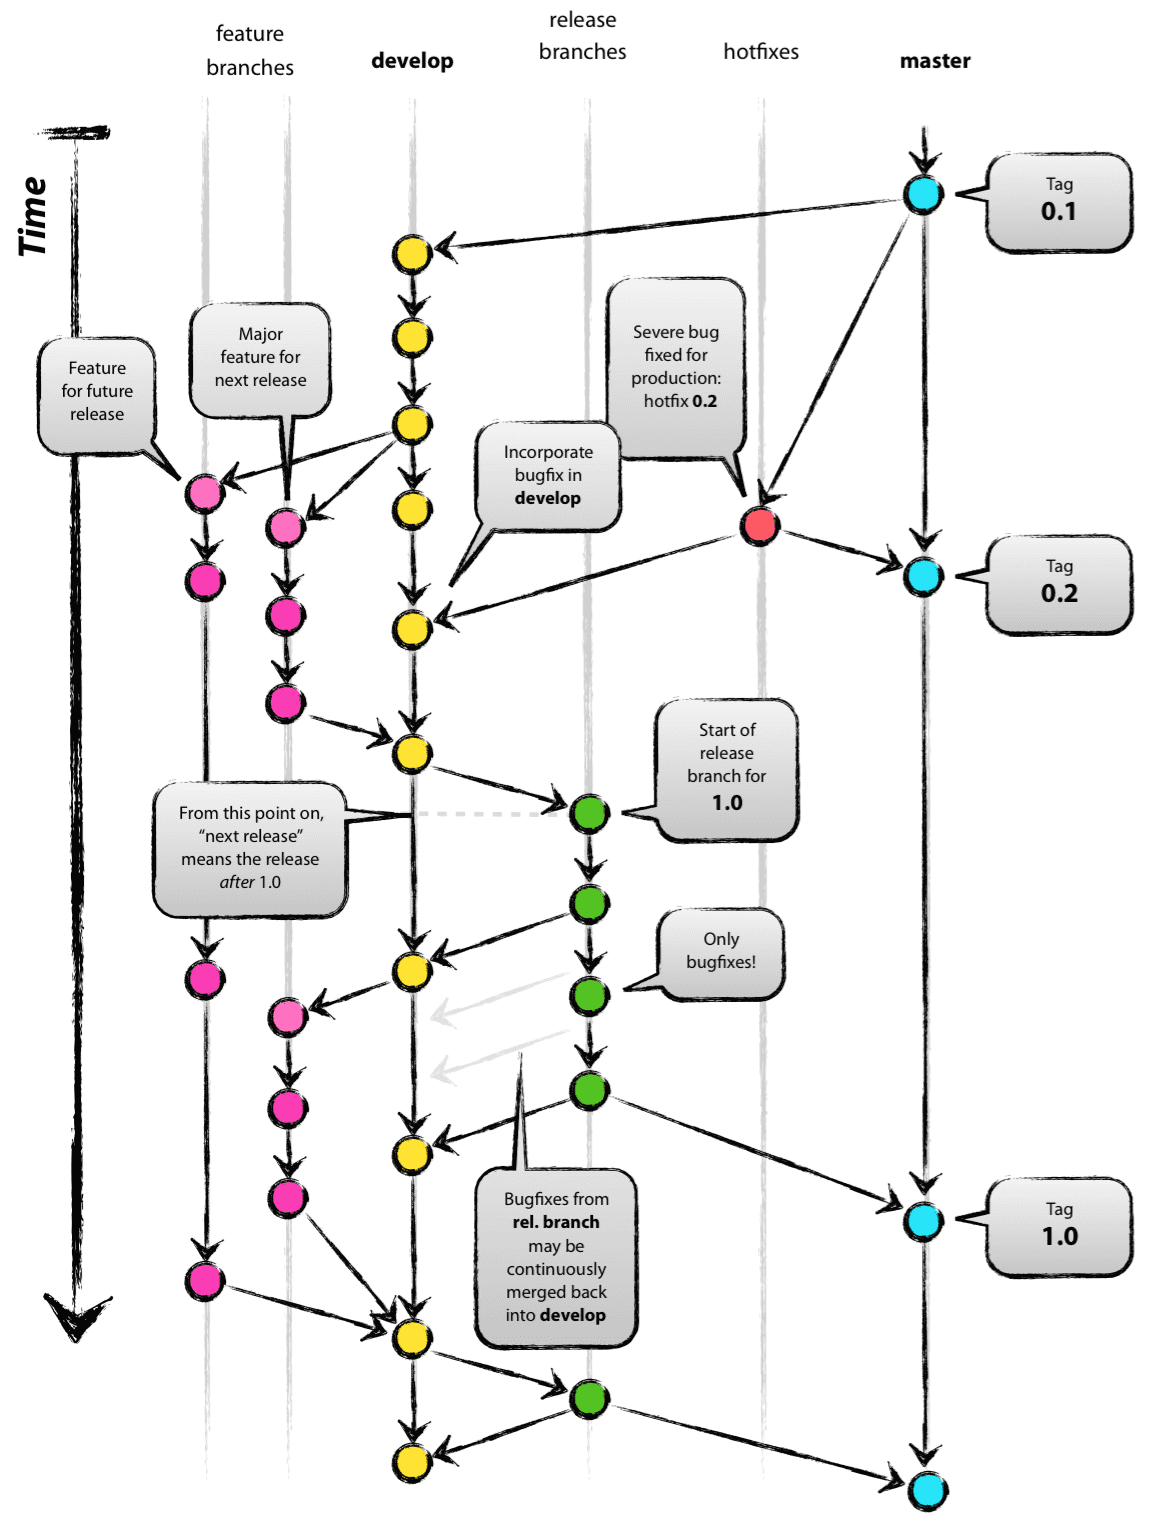
\includegraphics[scale=0.23]{./imagens/gitflow.png}%
        \end{center}%
        \caption{Diagrama da estratégia conhecida como GitFlow \label{fig:gitflow}}%
        \fonte{Vincent Driessen - \url{http://nvie.com/posts/a-successful-git-branching-model/} - Acessado em 01/03/2015}%
    \end{figure}%
    
O \textit{GitFlow} propõe que todos os desenvolvedores atuem diretamente no repositório principal do projeto, sendo que o trabalho é desenvolvido baseado em \textit{features} (recursos) e que o desenvolvimento de cada \textit{feature} é realizado num \textit{branch} criado especificamente para aquela feature. A integração das features é realizada num \textit{branch} chamado ``desenvolvimento'' e, de tempos em tempos, são fecha-se uma versão para publicação, que após integrada e testada é enviada ao \textit{branch} ``\textit{master}'', que conterá as versões estáveis do projeto, marcadas por meio de \textit{tags}.

Para se adequar à realidade da atual equipe de desenvolvimento da \gls{sal}, cada desenvolvedor deve realizar um \textit{fork} (bifurcação) do projeto dentro de seu próprio usuário do github e, em seguida, trabalhar utilizando o modelo do \textit{GitFlow} dentro de seu próprio \textit{fork}, utilizando o modelo de \textit{branches} proposto. Após a finalização de alguma \textit{feature}, a pessoa deve realizar um \textit{Pull-Request} de seu repositório para o repositório principal do projeto, para que este \textit{Pull-Request} possa ser avaliado pelo gestor do projeto e integrado ao repositório principal.

Outra modificação, necessária em função do legado já existente de trabalho do projeto, é que as integrações das \textit{features} ocorrerão no \textit{branch} ``master'', e não no ``desenvolvimento'', e as versões estáveis serão consolidadas no \textit{branch} ``stable''. Isso tanto no repositório principal quanto nos repositórios dos desenvolvedores.

Com isso, os desenvolvedores devem integrar suas features desenvolvidas em \textit{branches} no seu próprio repositório ``master'', realizar o \textit{Pull-request} para o repositório ``master'' do projeto principal e, no projeto principal, o \textit{branch} ``master'' será integrado ao ``stable'' com periodicidade a ser definida. A sequência abaixo resume este fluxo de trabalho, muito similar ao ``\textit{Forking Workflow}''\footnote{``\textit{Forking Workflow}'' - \url{https://www.atlassian.com/git/tutorials/comparing-workflows/forking-workflow} - Acessado em 12/03/2015}.
\newpage
\subsubsection{Passo a passo do \textit{workflow} de versionamento proposto}
Passo 1 - O gestor do projeto cria o repositório principal do projeto no ``servidor central'' (github)\footnote{No caso do presente projeto o serviço GitHub (\url{http://github.com}) será utilizado como servidor central dos repositórios de código do projeto}:
    \begin{figure}[htb]%
        \begin{center}
            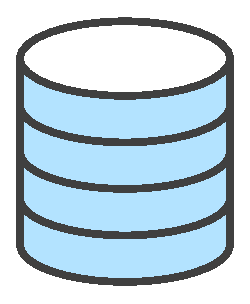
\includegraphics[scale=0.2]{./imagens/forkflow.eps}%
        \end{center}%
        \caption{Workflow de versionamento - passo 01 \label{fig:forkflow01}}%
        \fonte{Atlassian - Comparing Workflows - Acessado em 12/03/2015}%
    \end{figure}%

Passo 2 - Cada integrante da equipe de desenvolvimento cria seu próprio \textit{fork} no github:
    \begin{figure}[htb]%
        \begin{center}
            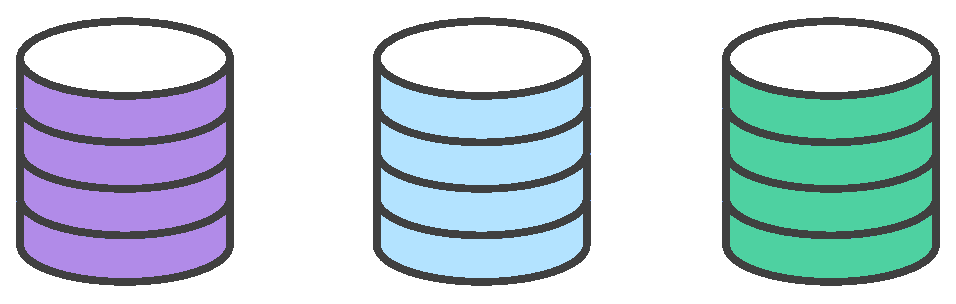
\includegraphics[scale=0.2]{./imagens/forkflow2.eps}%
        \end{center}%
        \caption{Workflow de versionamento - passo 02 \label{fig:forkflow02}}%
        \fonte{Atlassian - Comparing Workflows - Acessado em 12/03/2015}%
    \end{figure}%
    
Passo 3 - Cada integrante da equipe clona seu \textit{fork} em sua máquina local:
    \begin{figure}[htb]%
        \begin{center}
            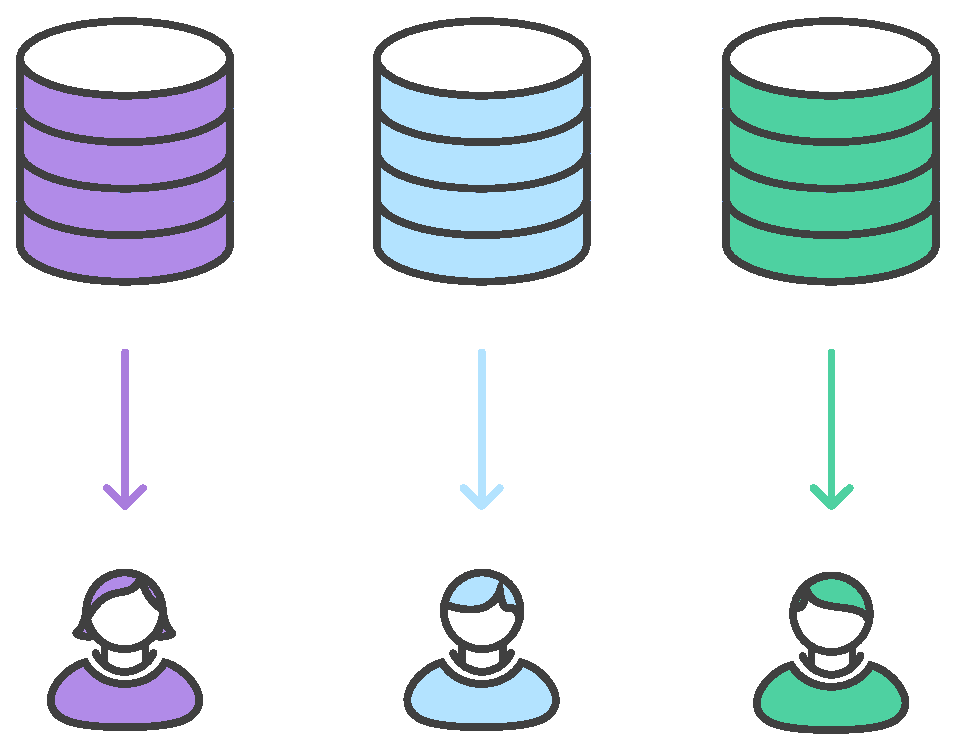
\includegraphics[scale=0.2]{./imagens/forkflow3.eps}%
        \end{center}%
        \caption{Workflow de versionamento - passo 03 \label{fig:forkflow03}}%
        \fonte{Atlassian - Comparing Workflows - Acessado em 12/03/2015}%
    \end{figure}%
\newpage
Passo 4 - Cada integrante da equipe desenvolve suas \textit{features} em \textit{branches} locais:
    \begin{figure}[htb]%
        \begin{center}
            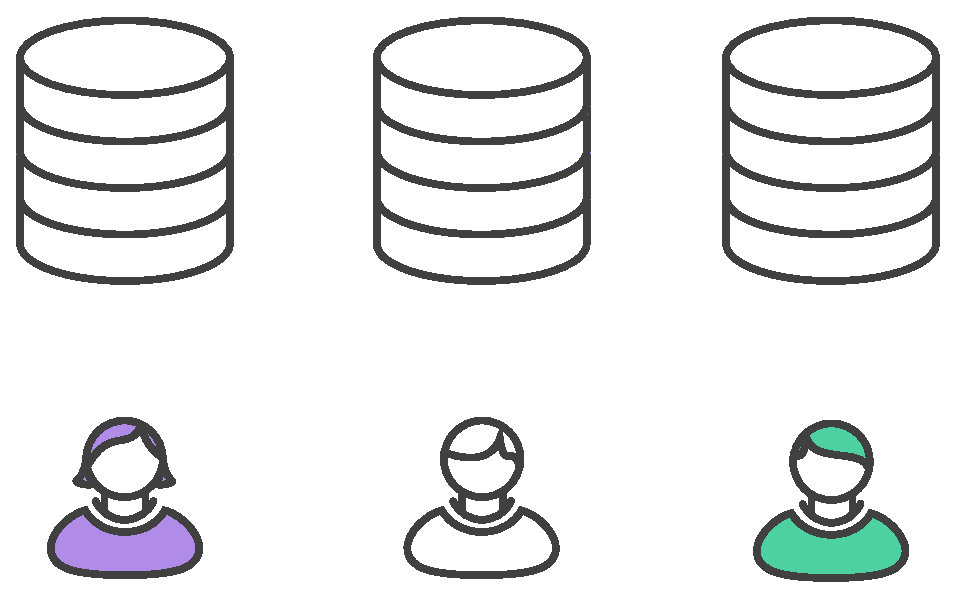
\includegraphics[scale=0.2]{./imagens/forkflow4.eps}%
        \end{center}%
        \caption{Workflow de versionamento - passo 04 \label{fig:forkflow04}}%
        \fonte{Atlassian - Comparing Workflows - Acessado em 12/03/2015}%
    \end{figure}%
    
Passo 5 - Após finalizada a \textit{feature}, o \textit{branch} da \textit{feature} é enviado para o repositório (\textit{fork}) do usuário no github. Caso haja mais de uma pessoa trabalhando na mesma \textit{feature}, recomenda-se que o \textit{branch} da \textit{feature} seja publicado constantemente ao \textit{fork} do usuário de forma que outro desenvolvedor possa utilizar as modificações feitas - realizando um \textit{pull} daquele \textit{branch} para seu repositório.
    \begin{figure}[htb]%
        \begin{center}
            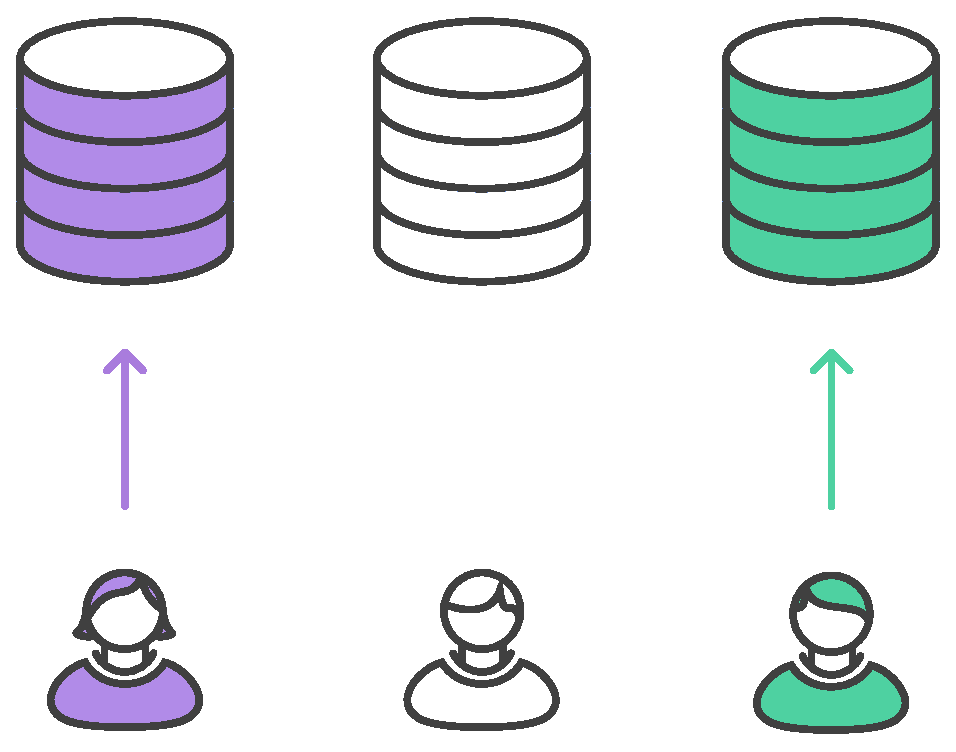
\includegraphics[scale=0.2]{./imagens/forkflow5.eps}%
        \end{center}%
        \caption{Workflow de versionamento - passo 05 \label{fig:forkflow05}}%
        \fonte{Atlassian - Comparing Workflows - Acessado em 12/03/2015}%
    \end{figure}%
\newpage
Passo 6 - Cada responsável por uma \textit{feature} realiza um \textit{Pull-Request} do \textit{branch} de sua \textit{feature} em seu \textit{fork} para o \textit{branch} ``master'' do repositório principal do projeto. Com os \textit{Pull-Requests} o gestor do projeto, no papel de integrador, verifica cada \textit{Pull-Request}, aceita (ou não) o \textit{Pull Request} e integra, uma a uma, as \textit{features} no repositório branch ``master'' de seu repositório local. Neste momento, cada \textit{Pull-Request} representará uma nova \textit{feature} (ou a resolução de algum \textit{bug}/\textit{issue}), e a cada integração deve-se realizar a validação da mesma.
    \begin{figure}[htb]%
        \begin{center}
            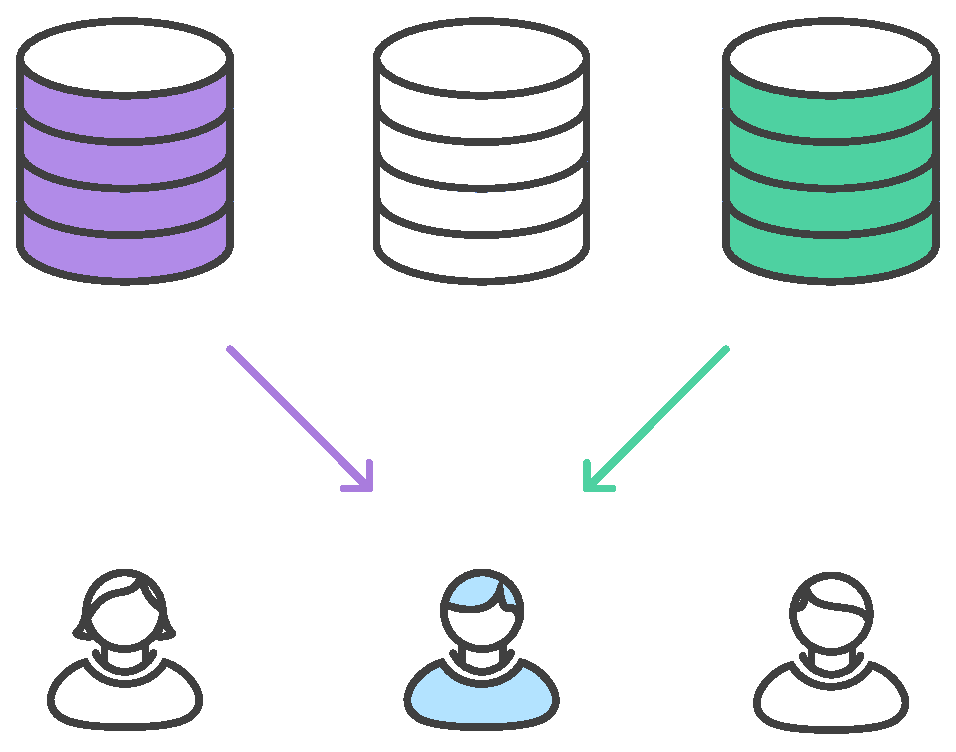
\includegraphics[scale=0.2]{./imagens/forkflow6.eps}%
        \end{center}%
        \caption{Workflow de versionamento - passo 06 \label{fig:forkflow06}}%
        \fonte{Autoria Própria}%
    \end{figure}%

Passo 7 - Após as integrações serem realizadas, o gestor deve enviar o \textit{branch} ``master'' de seu repositório local para o repositório principal do projeto.
    \begin{figure}[htb]%
        \begin{center}
            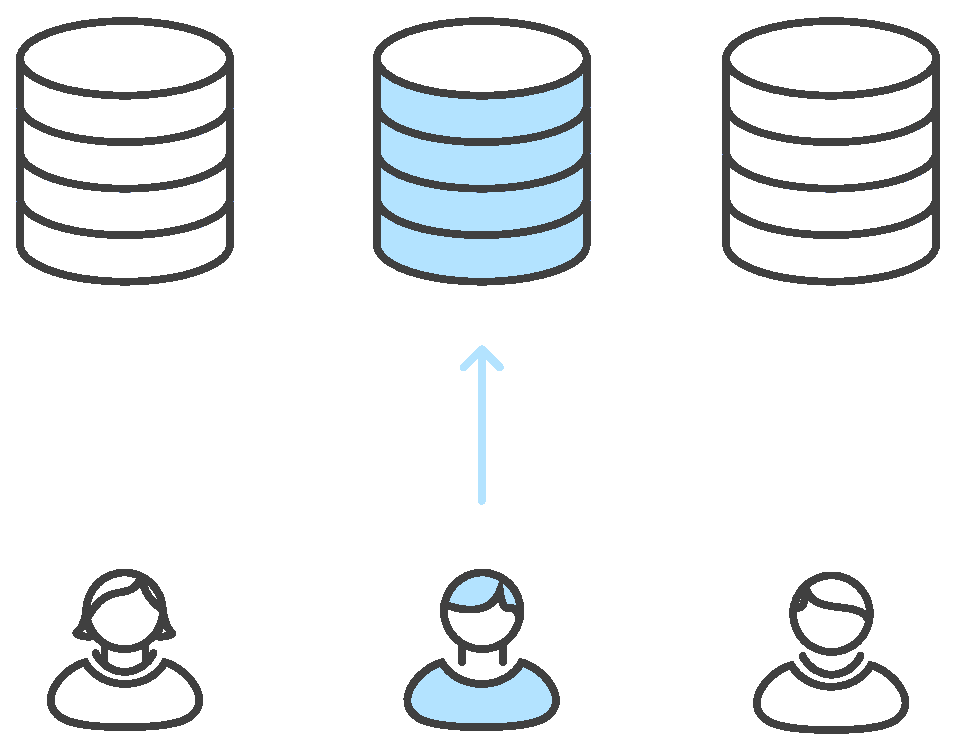
\includegraphics[scale=0.2]{./imagens/forkflow7.eps}%
        \end{center}%
        \caption{Workflow de versionamento - passo 07 \label{fig:forkflow07}}%
        \fonte{Autoria Própria}%
    \end{figure}%
\newpage
Passo 8 - Após a integração das \textit{features} ao repositório principal, todas pessoas que integram a equipe de desenvolvimento sincronizam novamente o \textit{branch} ``master'' de seus \textit{forks} com o \textit{branch} ``master'' do repositório principal.
    \begin{figure}[htb]%
        \begin{center}
            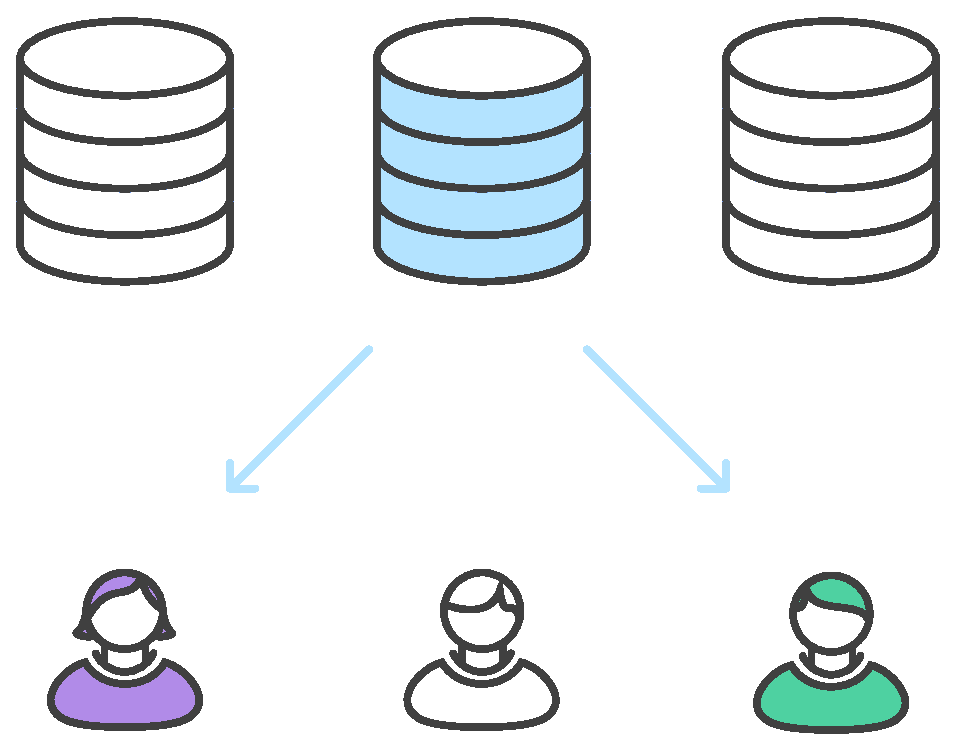
\includegraphics[scale=0.2]{./imagens/forkflow8.eps}%
        \end{center}%
        \caption{Workflow de versionamento - passo 08 \label{fig:forkflow08}}%
        \fonte{Atlassian - Comparing Workflows - Acessado em 12/03/2015}%
    \end{figure}%

Passo 9 - Periodicamente\footnote{A periodicidade depende do modelo de trabalho adotado, que não está definido neste processo de versionamento de código.}, após as integrações realizadas, o gestor define um \textit{release} e marca o repositório com uma \textit{tag} que defina tal \textit{release}, que em seguida será implementado no site em produção\footnote{O processo de implantação de novas versões em produção deve ser definido em outro documento.}.
    \begin{figure}[htb]%
        \begin{center}
            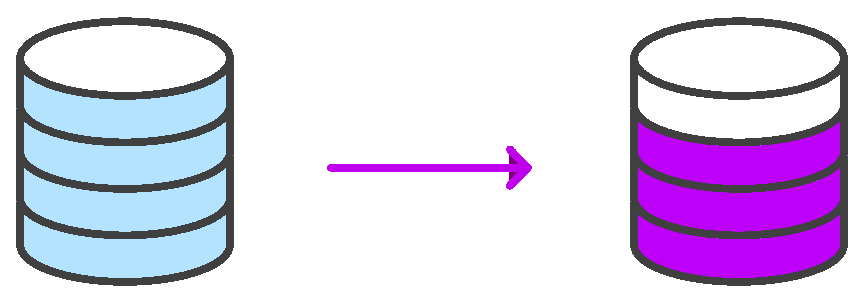
\includegraphics[scale=0.2]{./imagens/forkflow9.eps}%
        \end{center}%
        \caption{Workflow de versionamento - passo 09 \label{fig:forkflow09}}%
        \fonte{Atlassian - Comparing Workflows - Acessado em 12/03/2015}%
    \end{figure}%
